% ===== 第一部分：单变量分析学 / 第5章：级数理论 =====
% !TEX root = ../../main.tex
\setchapterimage{figure/chapter5封面图.png}
\setchapterintro{这一章我们的主题是级数，与我们的教材不同的是，我把级数的内容放在数列之后 ，因为我认为级数是一种特殊的数列，且两者确实能够互相转化。这一章我们研究的重点是级数的收敛性，而求级数具体的值，需要用到后续的积分，函数项级数之类的知识。}
\chapter{级数理论}
% 第1节：级数的定义
% !TEX root = ../../../main.tex
% 所属：第一部分：单变量分析学 / 第5章：级数理论
% 节：5.1 级数的定义
% 正文按原文件顺序保存；由 ../chapter5.tex 调用。
\section{级数的定义}
\begin{definition}
	形如 $a_1 + \dots + a_n + \dots$（$a_1, \dots, a_n, \dots \in \mathbb{R}$）叫作数项级数，记为 $\sum\limits_{n=1}^{\infty} a_n$，简写为 $\sum a_n$。
	
	由 $\sum a_n$ 可以构造一个部分和数列 $\{S_n\}_{n=1}^{\infty}$：
	\[
	S_n = \sum_{i=1}^{n} a_i
	\]
	
	称 $\sum a_n$ 收敛，当且仅当 $\{S_n\}$ 有一个有限的极限 $S$，称 $\sum a_n$ 收敛于 $S$，记为
	\[
	\sum_{n=1}^{\infty} a_n = S
	\]
	
\end{definition}

注意：不能通过 $S_n$ 的通项直接研究 $\sum a_n$，一般而言 $S_n$ 的通项难以求得，因此我们要从 $a_n$ 的角度研究 $\sum a_n$ 的收敛性。


\begin{example}
	\begin{enumerate}
		\item 等比级数 $1 + q + q^2 + \dots + q^n + \dots$
		
		部分和：
		\[
		S_n = 1 + \dots + q^{n-1} = \frac{1 - q^n}{1 - q}
		\]
		\begin{itemize}
			\item 当 $q = 1$ 时，$S_n = n \to +\infty$，级数发散；
			\item 当 $q = -1$ 时，$S_n$ 在 $0$ 和 $1$ 之间振荡，级数发散；
			\item 当 $|q| < 1$ 时，$S_n \to \dfrac{1}{1-q}$，级数收敛；
			\item 当 $|q| > 1$ 时，$S_n \to \infty$，级数发散。
		\end{itemize}
		\item $p$-级数
		\[
		\sum_{n=1}^{\infty} \frac{1}{n^p} = 1 + \frac{1}{2^p} + \dots + \frac{1}{n^p} + \dots
		\]
		
		部分和：
		\[
		S_n = 1 + \frac{1}{2^p} + \dots + \frac{1}{n^p}
		\]
		
		由 \ref{调和级数} 可知：
		\begin{itemize}
			\item 当 $p > 1$ 时，$\sum \dfrac{1}{n^p}$ 收敛；
			\item 当 $p \le 1$ 时，$\sum \dfrac{1}{n^p}$ 发散。
		\end{itemize}

	\end{enumerate}

\end{example}

\begin{proposition}(收敛的必要条件)
	若级数 $\sum a_n$ 收敛，则必有
	\[
	\lim_{n \to \infty} a_n = 0
	\]
	
\end{proposition}
\begin{proof}
	\[
	a_n = S_n - S_{n-1}
	\]
	由于 $\sum a_n$ 收敛，故部分和数列 $\{S_n\}$ 收敛，设
	\[
	\lim_{n \to \infty} S_n = S
	\]
	则同时有 $\lim\limits_{n \to \infty} S_{n-1} = S$，因此
	\[
	\lim_{n \to \infty} a_n = \lim_{n \to \infty} (S_n - S_{n-1}) = S - S = 0
	\]
\end{proof}
\begin{proposition}
	若级数 $\sum a_n$ 与 $\sum b_n$ 收敛，则对任意 $x,y \in \mathbb{R}$，级数 $\sum (x a_n + y b_n)$ 收敛，且
	\[
	\sum (x a_n + y b_n) = x \sum a_n + y \sum b_n
	\]
	
\end{proposition}

当 $\sum a_n$ 与 $\sum b_n$ 至少有一个发散时，上述结论不一定成立,例如：
 \begin{enumerate}
 	\item $a_n = \dfrac{1}{n}$，$b_n = -\dfrac{1}{n} + \dfrac{1}{n^2}$，此时 $\sum a_n$ 发散，$\sum b_n$ 发散，但 $\sum (a_n + b_n) = \sum \dfrac{1}{n^2}$ 收敛。
 	\item 又如：$a_n = \dfrac{1}{n}$，$b_n = \dfrac{1}{n}$，此时 $\sum a_n$、$\sum b_n$ 均发散，且 $\sum (a_n + b_n) = \sum \dfrac{2}{n}$ 也发散。
 	\item 若 $\sum a_n$ 发散，$\sum b_n$ 收敛，则 $\sum c_n = \sum (a_n + b_n)$ 必发散。（证明：用反证法。若 $\sum c_n$ 收敛，则 $\sum a_n = \sum c_n - \sum b_n$ 也收敛，与题设矛盾。）
 \end{enumerate}
\begin{proof}
	设 $S_n = \sum_{i=1}^{n} a_i$，$T_n = \sum_{i=1}^{n} b_i$，由 $\sum a_n$、$\sum b_n$ 收敛，可知
	\[
	\lim_{n \to \infty} S_n = S, \quad \lim_{n \to \infty} T_n = T
	\]
	而级数 $\sum (x a_n + y b_n)$ 的部分和为 $x S_n + y T_n$，于是
	\[
	\lim_{n \to \infty} (x S_n + y T_n) = xS + yT
	\]
	故 $\sum (x a_n + y b_n)$ 收敛，且结论得证。
\end{proof}


我们考虑级数上对加法的结合律与交换律。

对结合律：仅对收敛级数成立，发散级数不成立。

对交换律：对收敛级数也不一定成立。

例：对发散级数 $\sum (-1)^n$
\begin{align*}
	(-1+1)+(-1+1)+\dots &= 0+0+\dots = 0 \quad \text{收敛} \\
	-1+(1-1)+(1-1)+\dots &= -1+0+\dots = -1 \quad \text{收敛} \\
	(-1+1-1)+(1-1+1)+\dots &= -1+1-1+\dots \quad \text{发散}
\end{align*}
关于交换律的问题，我们后续再说。
\begin{proposition}
	设级数 $\sum a_n$ 收敛，则在其表达式 $a_1 + a_2 + \dots + a_n + \dots$ 中，不改变求和次序，任意添加括号（每个括号内为有限项），所得新级数也收敛，且其和与原级数相同。
\end{proposition}
\begin{proof}
	记原级数的部分和为 $S_n = a_1 + a_2 + \dots + a_n$。
	
	将原级数添加括号后，可表示为：
	\[
	\sum a_n = (a_1 + \dots + a_{n_1}) + (a_{n_1+1} + \dots + a_{n_2}) + \dots = b_1 + b_2 + \dots + b_k + \dots
	\]
	其中 $b_k = a_{n_{k-1}+1} + \dots + a_{n_k}$，约定 $n_0 = 0$。
	
	设新级数的部分和为 $T_k = b_1 + b_2 + \dots + b_k$，则有
	\[
	T_k = b_1 + \dots + b_k = S_{n_k}
	\]
	即 $\{T_k\}$ 是原级数部分和数列 $\{S_n\}$ 的一个子列。由于原级数收敛，$\{S_n\}$ 收敛，因此其子列 $\{T_k\}$ 也收敛，且极限相同。
	
	这就证明了新级数收敛，且和与原级数相同。
	
\end{proof}

%
% 第2节：正项级数
% !TEX root = ../../../main.tex
% 所属：第一部分：单变量分析学 / 第5章：级数理论
% 节：5.2 正项级数
% 正文按原文件顺序保存；由 ../chapter5.tex 调用。
\section{正项级数}
\begin{definition}
	若对级数 $\sum a_n$，存在 $N \in \mathbb{N}^+$，使得对所有 $n > N$，都有 $a_n > 0$，则称 $\sum a_n$ 为正项级数。
\end{definition}
\begin{proposition}
	一个正项级数收敛，当且仅当其部分和数列有界。
\end{proposition}
\begin{proof}
	根据单调有界收敛定理,显然
\end{proof}

\begin{proposition}\label{比较判别法}
	（比较判别法）对正项级数 $\sum x_n$ 与 $\sum y_n$，若存在常数 $A>0$ 与正整数 $N$，使得对所有 $n > N$，都有
	\[
	0 \le x_n \le A y_n
	\]
	则：
	\begin{enumerate}
		\item 若 $\sum y_n$ 收敛，则 $\sum x_n$ 收敛；
		\item 若 $\sum x_n$ 发散，则 $\sum y_n$ 发散。
	\end{enumerate}

	
\end{proposition}
\begin{proof}
	由于1和2互为逆否命题，我们只需证明1。
	
	设 $\sum x_n$ 的部分和为 $S_n$，$\sum y_n$ 的部分和为 $T_n$。
	已知 $\sum y_n$ 收敛，则其部分和数列 $\{T_n\}$ 有界，即存在常数 $M>0$，使得 $T_n \le M$ 对所有 $n$ 成立。
	
	对于 $n > N$，有
	\[
	0 \le x_n \le A y_n
	\]
	对 $n > N$ 求和可得：
	\[
	S_n = x_1 + \dots + x_N + x_{N+1} + \dots + x_n
	\le \sum_{k=1}^{N} x_k + A \sum_{k=N+1}^{n} y_k
	\]
	而
	\[
	\sum_{k=N+1}^{n} y_k = T_n - T_N \le T_n \le M
	\]
	因此
	\[
	0 \le S_n \le \sum_{k=1}^{N} x_k + A M
	\]
	这说明部分和数列 $\{S_n\}$ 单调上升且有上界，故 $\{S_n\}$ 收敛，即级数 $\sum x_n$ 收敛。
\end{proof}
\begin{corollary}
	（比较判别法的极限形式）设 $\sum x_n$ 与 $\sum y_n$ 为正项级数，且
	\[
	\lim_{n\to\infty} \frac{x_n}{y_n} = l
	\]
	
	则
	\begin{enumerate}
		\item 若 $0 \le l < +\infty$，且 $\sum y_n$ 收敛，则 $\sum x_n$ 收敛；
		\item 若 $0 < l \le +\infty$，且 $\sum x_n$ 发散，则 $\sum y_n$ 发散。
	\end{enumerate}
	
\end{corollary}
\begin{proof}
	取 $\varepsilon = 1$，由极限定义，存在 $N \in \mathbb{N}^+$，当 $n > N$ 时
	\[
	\left| \frac{x_n}{y_n} - l \right| < 1
	\]
	即
	\[
	l-1 < \frac{x_n}{y_n} < l+1
	\]
	
	\begin{itemize}
		\item 当 $0 \le l < +\infty$ 时，$x_n < (l+1)y_n$，由比较判别法，$\sum y_n$ 收敛 $\implies \sum x_n$ 收敛。
		\item 当 $0 < l \le +\infty$ 时，$x_n > (l-1)y_n$，由比较判别法，$\sum x_n$ 发散 $\implies \sum y_n$ 发散。
	\end{itemize}
	
	
	
	
\end{proof}
特别地，若 $0 < l < +\infty$，则 $\sum x_n$ 与 $\sum y_n$ 有相同的敛散性。
\begin{proposition}
	（Cauchy 判别法，根值判别法）
	设 $\sum\limits_{n=1}^{\infty} x_n$ 是正项级数，令
	\[
	r = \varlimsup_{n \to \infty} \sqrt[n]{x_n}
	\]
	
	则
	\begin{enumerate}
		\item 当 $r < 1$ 时，级数 $\sum x_n$ 收敛；
		\item 当 $r > 1$ 时，级数 $\sum x_n$ 发散；
		\item 当 $r = 1$ 时，级数可能收敛也可能发散。
	\end{enumerate}
	
\end{proposition}

对3：例如，调和级数 $\sum \dfrac{1}{n}$，此时 $r=1$，级数发散；而 $p$-级数 $\sum \dfrac{1}{n^2}$，此时 $r=1$，级数收敛。
\begin{proof}
	1.  当 $r < 1$ 时，取 $\varepsilon_0 = \dfrac{1-r}{2} > 0$，存在正整数 $N$，当 $n > N$ 时，有
	\[
	\sqrt[n]{x_n} < r + \varepsilon_0 = \frac{1+r}{2}
	\]
	即
	\[
	x_n < \left( \frac{1+r}{2} \right)^n
	\]
	由于 $0 < \dfrac{1+r}{2} < 1$，等比级数 $\sum \left( \dfrac{1+r}{2} \right)^n$ 收敛，由\ref{比较判别法}可知，级数 $\sum x_n$ 收敛。
	
	2.  当 $r > 1$ 时，取 $\varepsilon_0 = \dfrac{r-1}{2} > 0$，存在正整数 $N$，当 $n > N$ 时，有
	\[
	\sqrt[n]{x_n} > r - \varepsilon_0 = \frac{r+1}{2}
	\]
	即
	\[
	x_n > \left( \frac{r+1}{2} \right)^n
	\]
	由于 $\dfrac{r+1}{2} > 1$，等比级数 $\sum \left( \dfrac{r+1}{2} \right)^n$ 发散，由比较判别法可知，级数 $\sum x_n$ 发散。
\end{proof}




我们可以看到 Cauchy 判别法是包含 d'Alembert 判别法的，也就是说，能用 Cauchy 判别法的，d'Alembert 判别法可能失效；能用 d'Alembert 判别法的，理论上满足 Cauchy 判别法，依据是以下的命题。
\begin{proposition}\label{Cauchy 判别法是包含 d'Alembert 判别法}
	设 $\{x_n\}$ 是正项数列，则
	\[
	\varliminf_{n \to \infty} \frac{x_{n+1}}{x_n} \le \varliminf_{n \to \infty} \sqrt[n]{x_n} \le \varlimsup_{n \to \infty} \sqrt[n]{x_n} \le \varlimsup_{n \to \infty} \frac{x_{n+1}}{x_n}
	\]
\end{proposition}
\begin{proof}
	设
	\[
	\overline{r} = \varlimsup_{n \to \infty} \frac{x_{n+1}}{x_n}
	\]
	对任意 $\varepsilon > 0$，存在正整数 $N$，当 $n > N$ 时，有
	\[
	\frac{x_{n+1}}{x_n} < \overline{r} + \varepsilon
	\]
	于是
	\[
	x_n < (\overline{r} + \varepsilon)^{n-N-1} \cdot x_{N+1}
	\]
	从而
	\[
	\varlimsup_{n \to \infty} \sqrt[n]{x_n} \le \varlimsup_{n \to \infty} \sqrt[n]{(\overline{r} + \varepsilon)^{n-N-1} \cdot x_{N+1}} = \overline{r} + \varepsilon
	\]
	由 $\varepsilon$ 的任意性，得
	\[
	\varlimsup_{n \to \infty} \sqrt[n]{x_n} \le \overline{r} = \varlimsup_{n \to \infty} \frac{x_{n+1}}{x_n}
	\]
	
	对下极限的情况同理可证。
	
\end{proof}
\begin{proposition}
	（Raabe 判别法）设 $\sum x_n$ 为正项级数，且 $x_n \neq 0$，若极限
	\[
	\lim_{n \to \infty} n \left( \frac{x_n}{x_{n+1}} - 1 \right) = r
	\]
	存在且有限，则
	\begin{enumerate}
		\item 当 $r > 1$ 时，级数 $\sum x_n$ 收敛；
		\item 当 $r < 1$ 时，级数 $\sum x_n$ 发散。
	\end{enumerate}
	
\end{proposition}
\begin{proof}
	1.  当 $r > 1$ 时，取 $q = \dfrac{1+r}{2}$，则 $1 < q < r$。
	由极限定义，存在正整数 $N$，当 $n > N$ 时，有
	\[
	n \left( \frac{x_n}{x_{n+1}} - 1 \right) > q
	\]
	即
	\[
	\frac{x_n}{x_{n+1}} > 1 + \frac{q}{n}
	\]
	当 $n \to \infty$ 时，$\dfrac{1}{n} \to 0$，存在正整数 $N_2$，当 $n > N_2$ 时，有
	\[
	1 + \frac{q}{n} > \left( 1 + \frac{1}{n} \right)^{q_0}
	\]
	其中$q_0$略小于$q$,大于$1$，因此
	\[
	\frac{x_n}{x_{n+1}} > \left( 1 + \frac{1}{n} \right)^{q_0} = \frac{(n+1)^{q_0}}{n^{q_0}}
	\]
	即
	\[
	\frac{x_{n+1}}{x_n} < \frac{n^{q_0}}{(n+1)^{q_0}}
	\]
	递推可得
	\[
	x_{n+1} = \frac{x_{n+1}}{x_n} \cdot \frac{x_n}{x_{n-1}} \cdot \dots \cdot \frac{x_{N+2}}{x_{N+1}} \cdot x_{N+1} < \frac{(N+1)^{q_0}}{(n+1)^{q_0}} \cdot x_{N+1}
	\]
	由于 ${q_0} > 1$，$p$-级数 $\sum \dfrac{1}{n^{q_0}}$ 收敛，由比较判别法可知，级数 $\sum x_n$ 收敛。
	
	2.  当 $r < 1$ 时，取 $p = \dfrac{1+r}{2}$，则 $p < 1$。
	由极限定义，存在正整数 $N$，当 $n > N$ 时，有
	\[
	n \left( \frac{x_n}{x_{n+1}} - 1 \right) < p
	\]
	即
	\[
	\frac{x_n}{x_{n+1}} < 1 + \frac{p}{n} < \frac{n+1}{n}
	\]
	因此
	\[
	\frac{x_{n+1}}{x_n} > \frac{n}{n+1}
	\]
	递推可得
	\[
	x_{n+1} = \frac{x_{n+1}}{x_n} \cdot \dots \cdot \frac{x_{N+2}}{x_{N+1}} \cdot x_{N+1} > \frac{x_{N+1}}{n+1}
	\]
	由于调和级数 $\sum \dfrac{1}{n+1}$ 发散，由比较判别法可知，级数 $\sum x_n$ 发散。
	
	
\end{proof}



\begin{proposition}
	（高斯判别法）
	设 $\sum\limits_{n=1}^{\infty} x_n$ 为正项级数，且 $x_n>0$。
	若存在常数 $\alpha$ 和 $\lambda>1$，使得
	\[
	\frac{x_n}{x_{n+1}}
	=
	1+\frac{\alpha}{n}+O\left(\frac{1}{n^\lambda}\right),
	\qquad n\to\infty,
	\]
	则有
	\[
	\begin{cases}
		\alpha>1, & \displaystyle \sum_{n=1}^{\infty}x_n \text{ 收敛},\\[6pt]
		\alpha\leq 1, & \displaystyle \sum_{n=1}^{\infty}x_n \text{ 发散}.
	\end{cases}
	\]
\end{proposition}
若
\[
\frac{x_n}{x_{n+1}}
=
1+\frac{\alpha}{n}+O\left(\frac{1}{n^\lambda}\right),
\qquad \lambda>1,
\]
则
\[
n\left(\frac{x_n}{x_{n+1}}-1\right)
=
\alpha+O\left(\frac{1}{n^{\lambda-1}}\right).
\]
因为 $\lambda>1$，所以
\[
O\left(\frac{1}{n^{\lambda-1}}\right)\to 0.
\]
于是
\[
\lim_{n\to\infty}
n\left(\frac{x_n}{x_{n+1}}-1\right)
=
\alpha.
\]
因此，当 $\alpha>1$ 或 $\alpha<1$ 时，Raabe 判别法已经可以判断级数的敛散性。
高斯判别法的意义在于，它还可以处理临界情形 $\alpha=1$，
并进一步给出发散结论。


\begin{lemma}
设 $\{z_n\}$ 为正项数列。若
\[
\frac{z_n}{z_{n+1}}=1+\varepsilon_n,
\]
且$\sum\limits_{n=1}^{\infty}|\varepsilon_n|$收敛，则存在常数 $L>0$，使得
\[
\lim_{n\to\infty} z_n=L.
\]
\end{lemma}
\begin{proof}
	由于$\sum\limits_{n=1}^{\infty}|\varepsilon_n|$
收敛，所以$\varepsilon_n\to 0.$因此存在正整数 $N$，当 $n>N$ 时，$|\varepsilon_n|<\frac12.$于是 $1+\varepsilon_n>0$，并且 $\ln(1+\varepsilon_n)$ 有意义。

当 $|t|<\dfrac12$ 时，
\[
|\ln(1+t)|\leq 2|t|.
\]
所以
\[
\sum_{n=N}^{\infty}|\ln(1+\varepsilon_n)|
\leq
2\sum_{n=N}^{\infty}|\varepsilon_n|
<+\infty.
\]
故级数$\sum_{n=N}^{\infty}\ln(1+\varepsilon_n)$收敛。

由
\[
\frac{z_n}{z_{n+1}}=1+\varepsilon_n
\]
可得
\[
\ln z_{n+1}
=
\ln z_n-\ln(1+\varepsilon_n).
\]
于是递推得到
\[
\ln z_n
=
\ln z_N-\sum_{k=N}^{n-1}\ln(1+\varepsilon_k).
\]
由于右端的级数收敛，所以 $\ln z_n$ 收敛于某个有限实数。
设
\[
\ln z_n\to \ln L,
\]
则
\[
z_n\to L.
\]
又因为 $z_n>0$，所以 $L>0$。
引理得证。
\end{proof}



下面证明高斯判别法。

\begin{proof}
	由条件可知
\[
\frac{x_n}{x_{n+1}}
=
1+\frac{\alpha}{n}+O\left(\frac{1}{n^\lambda}\right),
\qquad \lambda>1.
\]

构造新的正项数列
\[
z_n=n^\alpha x_n.
\]
则
\[
\frac{z_n}{z_{n+1}}
=
\frac{n^\alpha x_n}{(n+1)^\alpha x_{n+1}}
=
\left(\frac{n}{n+1}\right)^\alpha
\frac{x_n}{x_{n+1}}.
\]
因此
\[
\frac{z_n}{z_{n+1}}
=
\left(1+\frac{1}{n}\right)^{-\alpha}
\left[
1+\frac{\alpha}{n}
+
O\left(\frac{1}{n^\lambda}\right)
\right].
\]

由 Taylor 展开可得
\[
\left(1+\frac{1}{n}\right)^{-\alpha}
=
1-\frac{\alpha}{n}
+
O\left(\frac{1}{n^2}\right).
\]
于是
\[
\frac{z_n}{z_{n+1}}
=
\left[
1-\frac{\alpha}{n}
+
O\left(\frac{1}{n^2}\right)
\right]
\left[
1+\frac{\alpha}{n}
+
O\left(\frac{1}{n^\lambda}\right)
\right].
\]
展开得
\[
\frac{z_n}{z_{n+1}}
=
1
+
O\left(\frac{1}{n^2}\right)
+
O\left(\frac{1}{n^\lambda}\right).
\]

令$\rho=\min\{2,\lambda\}.$因为 $\lambda>1$，所以$\rho>1.$因此
\[
\frac{z_n}{z_{n+1}}
=
1+O\left(\frac{1}{n^\rho}\right),
\qquad \rho>1.
\]
即存在数列 $\varepsilon_n$，使得
\[
\frac{z_n}{z_{n+1}}=1+\varepsilon_n,
\]
且$|\varepsilon_n|\leq \dfrac{C}{n^\rho}.$由于$\sum\limits_{n=1}^{\infty}\dfrac{1}{n^\rho}$收敛，所以$\sum\limits_{n=1}^{\infty}|\varepsilon_n|$收敛。

由引理可知，存在常数 $L>0$，使得$z_n\to L.$即$n^\alpha x_n\to L.$因此
\[
x_n\sim \frac{L}{n^\alpha}.
\]

于是由
\[
\sum_{n=1}^{\infty}\frac{1}{n^\alpha}
\begin{cases}
	\text{收敛}, & \alpha>1,\\
	\text{发散}, & \alpha\leq 1.
\end{cases}
\]
所以
\[
\sum_{n=1}^{\infty}x_n
\begin{cases}
	\text{收敛}, & \alpha>1,\\
	\text{发散}, & \alpha\leq 1.
\end{cases}
\]
高斯判别法得证。
\end{proof}




\begin{proposition}
	（Cauchy 凝聚判别法）
	对正项级数 $\sum a_n$，若 $\{a_n\}$ 单调递减，则级数 $\sum a_n$ 收敛，当且仅当级数
	\[
	\sum_{k=0}^{\infty} 2^k a_{2^k} = a_1 + 2a_2 + 4a_4 + \dots
	\]
	收敛。
\end{proposition}
\begin{proof}
	只需考虑 $\sum a_n$ 与 $\sum 2^k a_{2^k}$ 的部分和是否有界即可。
	设原级数的部分和为 $S_n = a_1 + a_2 + \dots + a_n$，
	凝聚级数的部分和为 $T_k = a_1 + 2a_2 + \dots + 2^k a_{2^k}$。
	
	当 $n < 2^k$ 时，
	\[
	\begin{aligned}
		S_n &\le a_1 + (a_2 + a_3) + \dots + (a_{2^k} + \dots + a_{2^{k+1}-1}) \\
		&\le a_1 + 2a_2 + \dots + 2^k a_{2^k} = T_k
	\end{aligned}
	\]
	即
	\[
	S_n \le T_k \tag{1}
	\]
	
	当 $n > 2^k$ 时，
	\[
	\begin{aligned}
		S_n &\ge a_1 + a_2 + (a_3 + a_4) + \dots + (a_{2^{k-1}+1} + \dots + a_{2^k}) \\
		&\ge \frac{1}{2}a_1 + a_2 + 2a_4 + \dots + 2^{k-1}a_{2^k} = \frac{1}{2}T_k
	\end{aligned}
	\]
	因此
	\[
	2S_n \ge T_k \tag{2}
	\]
	
	由 (1) 和 (2) 可知，部分和数列 $\{S_n\}$ 与 $\{T_k\}$ 同时有界或同时无界，故原级数与凝聚级数具有相同的敛散性。
\end{proof}
\begin{lemma}\label{级数1/nlnn}
	级数 $\sum\limits_{n=2}^{\infty} \dfrac{1}{n(\ln n)^p}$ 当 $p>1$ 时收敛，当 $p \le 1$ 时发散。
\end{lemma}
\begin{proof}
	对
	\[
	a_n = \frac{1}{n(\ln n)^p}
	\]
	$\{a_n\}$ 单调递减，计算
	\[
	2^k a_{2^k} = 2^k \cdot \frac{1}{2^k (\ln 2^k)^p} = \frac{1}{(k \ln 2)^p} = \frac{1}{(\ln 2)^p} \cdot \frac{1}{k^p}
	\]
	那么
	\[
	\sum_{k=1}^{\infty} 2^k a_{2^k} = \frac{1}{(\ln 2)^p} \cdot \sum_{k=1}^{\infty} \frac{1}{k^p}
	\]
	这是 $p$-级数，故当 $p > 1$ 时收敛，当 $ p \le 1$ 时发散。
	
\end{proof}

类似地，
\[
\sum_{n=3}^{\infty} \frac{1}{n \ln n \cdot \ln \ln n} \quad \text{发散},
\]
\[
\sum_{n=3}^{\infty} \frac{1}{n \ln n (\ln \ln n)^2} \quad \text{收敛}.\]
\begin{proposition}
	（Bertrand 判别法）对正项级数 $\sum x_n$，设
	\[
	\lim_{n \to \infty} (\ln n) \left[ n \left( \frac{x_n}{x_{n+1}} - 1 \right) - 1 \right] = r
	\]
	则
	\begin{itemize}
		\item 当 $r > 1$ 时，级数 $\sum x_n$ 收敛；
		\item 当 $r < 1$ 时，级数 $\sum x_n$ 发散。
	\end{itemize}

\end{proposition}
\begin{proof}
	考虑级数 $\sum \dfrac{1}{n(\ln n)^p}$，设 $y_n = \dfrac{1}{n(\ln n)^p}$，则
	\[
	\frac{y_n}{y_{n+1}} = \left(1 + \frac{1}{n}\right) \left( \frac{\ln(n+1)}{\ln n} \right)^p
	\]
	利用 Taylor 展开，
	\[
	\ln(n+1) = \ln n + \ln\left(1+\frac{1}{n}\right) = \ln n + \frac{1}{n} - \frac{1}{2n^2} + O\left(\frac{1}{n^3}\right)
	\]
	因此
	\[
	\left( \frac{\ln(n+1)}{\ln n} \right)^p = \left( 1 + \frac{1}{n \ln n} - \frac{1}{2n^2 \ln n} + \dots \right)^p = 1 + \frac{p}{n \ln n} + o\left( \frac{1}{n \ln n} \right)
	\]
	从而
	\[
	\frac{y_n}{y_{n+1}} = 1 + \frac{1}{n} + \frac{p}{n \ln n} + o\left( \frac{1}{n \ln n} \right)
	\]
	整理得
	\[
	n \left( \frac{y_n}{y_{n+1}} - 1 \right) - 1 = \frac{p}{\ln n} + o\left( \frac{1}{\ln n} \right)
	\]
	因此
	\[
	\lim_{n \to \infty} (\ln n) \left[ n \left( \frac{y_n}{y_{n+1}} - 1 \right) - 1 \right] = p
	\]
	
	1.  当 $r > 1$ 时，取 $p$ 使得 $1 < p < r$，则 $\sum y_n$ 收敛，且
	\[
	\lim_{n \to \infty} (\ln n) \left[ n \left( \frac{y_n}{y_{n+1}} - 1 \right) - 1 \right] = p < r
	\]
	考虑$x_n$与$y_n$相邻项之比的差
	\[
	(\ln n) \left[ n \left( \frac{x_n}{x_{n+1}} - 1 \right) - 1 \right]-(\ln n) \left[ n \left( \frac{y_n}{y_{n+1}} - 1 \right) - 1 \right] = n \ln n (\frac{x_n}{x_{n+1}} -\frac{y_n}{y_{n+1}} )
	\]
	由极限的保号性，存在正整数 $N$，当 $n > N$ 时，有
	\[
	\frac{x_n}{x_{n+1}} > \frac{y_n}{y_{n+1}} \implies \frac{x_{n+1}}{x_n} < \frac{y_{n+1}}{y_n}
	\]
	递推可得，当 $n > N$ 时
	\[
	\frac{x_n}{x_N} < \frac{y_n}{y_N} \implies x_n < \frac{x_N}{y_N} y_n
	\]
	由于 $\sum y_n$ 收敛，由比较判别法可知 $\sum x_n$ 收敛。
	
	2.  当 $r < 1$ 时，取 $p$ 使得 $r < p < 1$，则 $\sum y_n$ 发散，同理，由极限的保号性，存在正整数 $N$，当 $n > N$ 时
	\[
	x_n > \frac{x_N}{y_N} y_n
	\]
	由于 $\sum y_n$ 发散，故 $\sum x_n$ 发散。
	
\end{proof}












%
% 第3节：任意项级数
% !TEX root = ../../../main.tex
% 所属：第一部分：单变量分析学 / 第5章：级数理论
% 节：5.3 任意项级数
% 正文按原文件顺序保存；由 ../chapter5.tex 调用。
\section{任意项级数}
这节我们研究不规定 $x_n$ 正负的任意项级数。
\begin{proposition}
	（Cauchy 收敛准则）
	级数 $\sum x_n$ 收敛，当且仅当对任意 $\varepsilon > 0$，存在正整数 $N$，使得对所有 $n > N$ 和所有正整数 $p \ge 1$，都有
	\[
	|x_{n+1} + x_{n+2} + \dots + x_{n+p}| < \varepsilon
	\]
\end{proposition}
\begin{proof}
	由数列的 Cauchy 收敛准则易得。
\end{proof}

类似地，我们有 Cauchy 不收敛准则。

\begin{definition}
	形如
	\[
	\sum_{n=1}^{\infty} (-1)^n a_n \quad (a_n > 0)
	\]
	的级数，称为交错级数。
	在交错级数中，若数列 $\{a_n\}$ 单调递减且 $\lim\limits_{n \to \infty} a_n = 0$，则称为 Leibniz 级数。
\end{definition}
\begin{proposition}\label{Leibniz 级数必然收敛。}
	Leibniz 级数必然收敛。
\end{proposition}

\begin{proof}
	设 $\sum x_n$ 为 Leibniz 级数，即 $x_n = (-1)^n u_n$，其中 $u_n > 0$，且数列 $\{u_n\}$ 单调递减并趋于 $0$。
	
	对任意 $n \in \mathbb{N}$ 和任意正整数 $p \ge 1$，考虑
	\[
	\begin{aligned}
		|x_{n+1} + x_{n+2} + \dots + x_{n+p}|
		&= |(-1)^{n+1} u_{n+1} + (-1)^{n+2} u_{n+2} + \dots + (-1)^{n+p} u_{n+p}| \\
		&= |u_{n+1} - u_{n+2} + u_{n+3} - \dots + (-1)^{p-1} u_{n+p}|
	\end{aligned}
	\]
	
	若 $p$ 为偶数，则
	\[
	\begin{aligned}
		|x_{n+1} + \dots + x_{n+p}|
		&= |(u_{n+1} - u_{n+2}) + (u_{n+3} - u_{n+4}) + \dots + (u_{n+p-1} - u_{n+p})| \\
		&= (u_{n+1} - u_{n+2}) + (u_{n+3} - u_{n+4}) + \dots + (u_{n+p-1} - u_{n+p}) \\
		&= u_{n+1} - (u_{n+2} - u_{n+3}) - \dots - (u_{n+p-2} - u_{n+p-1}) - u_{n+p} \\
		&\le u_{n+1}
	\end{aligned}
	\]
	
	由于 $\lim\limits_{n \to \infty} u_n = 0$，对任意 $\varepsilon > 0$，存在正整数 $N$，当 $n > N$ 时，有 $0 < u_{n+1} < \varepsilon$，因此
	\[
	|x_{n+1} + \dots + x_{n+p}| \le u_{n+1} < \varepsilon
	\]
	
	对 $p$ 为奇数的情况，同理可得
	\[
	|x_{n+1} + \dots + x_{n+p}| < u_{n+1} < \varepsilon
	\]
	
	由 Cauchy 收敛准则可知，Leibniz 级数 $\sum x_n$ 收敛。
	
\end{proof}
\begin{example}
	级数
	\[\sum_{n=1}^\infty\frac{(-1)^n}{n^p}\]
	在$p>0$时收敛
	
	但
	\[\sum_{n=1}^\infty\frac{1}{n^p}\]未必
\end{example}
在\ref{Leibniz 级数必然收敛。}的证明中，我们得到以下结论
\begin{proposition}
	（Leibniz 级数的余项估计）
	设 $\sum x_n$ 为 Leibniz 级数，即 $x_n = (-1)^n u_n$，其中 $u_n > 0$，数列 $\{u_n\}$ 单调递减且趋于 $0$。
	记余项
	\[
	r_n = \left| \sum_{k=1}^{\infty} (-1)^k u_k - S_n \right| = \left| \sum_{k=n+1}^{\infty} (-1)^k u_k \right|
	\]
	则有
	\[
	r_n \le u_{n+1}
	\]
	即截断误差小于截断后的第一项的绝对值。
\end{proposition}
\begin{lemma}
	（Abel 引理）
	对数列 $\{a_n\}$ 与 $\{b_n\}$，设 $B_k = \sum_{i=1}^k b_i$ 为 $\{b_n\}$ 的部分和。若满足：
	\begin{enumerate}
		\item 数列 $\{a_k\}$ 单调； 
		\item 部分和数列 $\{B_k\}$ 有界，即存在常数 $M > 0$，使得对所有 $k$，有 $|B_k| \le M$。
	\end{enumerate}

	则
	\[
	\left| \sum_{k=1}^p a_k b_k \right| \le M \left( |a_1| + 2|a_p| \right)
	\]
\end{lemma}
\begin{proof}
	由 Abel 变换，
	\[
	\sum_{k=1}^p a_k b_k = a_p B_p + \sum_{k=1}^{p-1} (a_k - a_{k+1}) B_k
	\]
	因此
	\[
	\begin{aligned}
		\left| \sum_{k=1}^p a_k b_k \right|
		&= \left| a_p B_p + \sum_{k=1}^{p-1} (a_k - a_{k+1}) B_k \right| \\
		&\le |a_p| |B_p| + |\sum_{k=1}^{p-1} a_k - a_{k+1}| |B_k| \\
		&\le M |a_p| + M |\sum_{k=1}^{p-1} a_k - a_{k+1}|
	\end{aligned}
	\]
	$|\sum\limits_{k=1}^{p-1} a_k - a_{k+1}| = |a_1 - a_p|$，故
	\[
	\left| \sum_{k=1}^p a_k b_k \right| \le M |a_p| + M |a_1 - a_p| \le M \left( |a_1| + 2|a_p| \right)
	\]
	
\end{proof}
\begin{proposition}
	（级数的 Abel-Dirichlet 判别法）
	对级数 $\sum a_n b_n$，满足以下条件之一时级数收敛：
	
	\begin{enumerate}
		\item \textbf{Abel 判别法}：数列 $\{a_n\}$ 单调有界，级数 $\sum b_n$ 收敛。
		\item \textbf{Dirichlet 判别法}：数列 $\{a_n\}$ 单调趋于 $0$，且部分和数列 $\{B_n\}$ 有界
	\end{enumerate}
\end{proposition}
\begin{proof}
	\begin{enumerate}
		\item \textbf{Abel 判别法}
		
		由 $\{a_n\}$ 有界，存在常数 $L > 0$，使得对所有 $n$，有 $|a_n| \le L$。
		又由 $\sum b_n$ 收敛，根据 Cauchy 收敛准则，对任意 $\varepsilon > 0$，存在正整数 $N$，当 $n > N$ 且 $p \ge 1$ 时，有
		\[
		|b_{n+1} + b_{n+2} + \dots + b_{n+p}| < \varepsilon
		\]
		由 Abel 引理，
		\[
		|a_{n+1}b_{n+1} + \dots + a_{n+p}b_{n+p}| \le \varepsilon(|a_{n+1}| + 2|a_{n+p}|) \le \varepsilon(L + 2L) = 3L\varepsilon
		\]
		由 Cauchy 收敛准则，级数 $\sum a_n b_n$ 收敛。
		
		\item \textbf{Dirichlet 判别法}
		
		由 $\{B_n\}$ 有界，存在常数 $M > 0$，使得对所有 $n$，有 $|B_n| \le M$。
		因此，任意部分和 $|\widetilde{B}_k| = |b_{n+1} + \dots + b_{n+p}| = |B_{n+p} - B_n| \le |B_{n+p}| + |B_n| \le 2M$。
		又由 $a_n \to 0$，对任意 $\varepsilon > 0$，存在正整数 $N$，当 $n > N$ 时，$|a_n| < \varepsilon$。
		再由 $\{a_n\}$ 单调及 Abel 引理，
		\[
		\left| \sum_{k=n+1}^{n+p} a_k b_k \right| \le 2M \big( |a_{n+1}| + 2|a_{n+p}| \big) < 2M(\varepsilon + 2\varepsilon) = 6M\varepsilon
		\]
		由 Cauchy 收敛准则，级数 $\sum a_n b_n$ 收敛。
	\end{enumerate}
	
\end{proof}
%
% 第4节：级数的绝对收敛与条件收敛
% !TEX root = ../../../main.tex
% 所属：第一部分：单变量分析学 / 第5章：级数理论
% 节：5.4 级数的绝对收敛与条件收敛
% 正文按原文件顺序保存；由 ../chapter5.tex 调用。
\section{级数的绝对收敛与条件收敛}
\begin{definition}
	对级数 $\sum a_n$，若级数 $\sum |a_n|$ 收敛，则称级数 $\sum a_n$ \text{绝对收敛}。
	
	由不等式
	\[
	|a_{n+1} + a_{n+2} + \dots + a_{n+p}| \le |a_{n+1}| + |a_{n+2}| + \dots + |a_{n+p}| < \varepsilon
	\]
	可知：\text{绝对收敛的级数必收敛}。
	若级数 $\sum a_n$ 收敛，但不绝对收敛，则称级数 $\sum a_n$ 条件收敛。
\end{definition}

\begin{example}
	讨论级数 $\displaystyle \sum_{n=1}^{\infty} \frac{x^n}{n^p}$ 的敛散性
	
\end{example}
\begin{solution}
	对其绝对值级数
	\[
	\sum_{n=1}^{\infty} \left| \frac{x^n}{n^p} \right| = \sum_{n=1}^{\infty} \frac{|x|^n}{n^p}
	\]
	应用 Cauchy 判别法：
	\[
	\lim_{n \to \infty} \sqrt[n]{\frac{|x|^n}{n^p}} = |x|
	\]
	
	\begin{itemize}
		\item 若 $|x| < 1$，对任意 $p \in \mathbb{R}$，级数绝对收敛。
		\item 若 $|x| > 1$，对任意 $p \in \mathbb{R}$，级数发散。
	\end{itemize}
	
	接下来讨论边界情况：
	
	\begin{itemize}
		\item \text{当 $x=1$ 时}：级数为 $\displaystyle \sum_{n=1}^{\infty} \frac{1}{n^p}$，即 $p$-级数：
		\begin{itemize}
			\item $p > 1$：级数绝对收敛；
			\item $p \le 1$：级数发散。
		\end{itemize}
		
		\item \text{当 $x=-1$ 时}：级数为 $\displaystyle \sum_{n=1}^{\infty} \frac{(-1)^n}{n^p}$：
		\begin{itemize}
			\item $p > 1$：级数绝对收敛；
			\item $0 < p \le 1$：级数条件收敛（由 Leibniz 判别法）；
			\item $p \le 0$：级数发散（通项不趋于0）。
		\end{itemize}
	\end{itemize}
	
\end{solution}
\begin{definition}
	将级数 $\sum x_n$ 求和中的数列 $\{x_n\}$ 的次序重新排列，但不新增也不遗漏。
	
	设所得的数列为 $\{x'_n\}$，对应的级数为 $\sum x'_n$，称之为 $\sum x_n$ 的 \text{更序级数}。
	$\sum x_n$ 也为 $\sum x'_n$ 的更序级数，称这一过程为 \text{级数的重排}。
\end{definition}
\begin{example}
	考虑级数
	\[
	\sum_{n=1}^{\infty} \frac{(-1)^{n+1}}{n} = \ln 2
	\]
	的重排：
	\[
	1 - \frac{1}{2} - \frac{1}{4} + \frac{1}{3} - \frac{1}{6} - \frac{1}{8} + \dots = \sum x'_n
	\]
\end{example}

\begin{solution}
	设原级数的部分和为 $S_n = \sum\limits_{k=1}^{n} \dfrac{(-1)^{k+1}}{k}$。
	重排级数的部分和
	\[
	\begin{aligned}
		S'_{3n} &= 1 - \frac{1}{2} - \frac{1}{4} + \dots + \left( \frac{1}{2n-1} - \frac{1}{4n-2} - \frac{1}{4n} \right) \\
		&= \sum_{k=1}^{n} \left( \frac{1}{4k-2} - \frac{1}{4k} \right) \\
		&= \frac{1}{2} \sum_{k=1}^{n} \left( \frac{1}{2k-1} - \frac{1}{2k} \right) \\
		&= \frac{1}{2} \left( 1 - \frac{1}{2} + \frac{1}{3} - \frac{1}{4} + \dots \right) = \frac{1}{2} S_{2n} \to \frac{1}{2} \ln 2
	\end{aligned}
	\]
	而
	\[
	S'_{3n-1} = S'_{3n} + \frac{1}{4n} \to \frac{1}{2} \ln 2
	\]
	\[
	S'_{3n-2} = S'_{3n} + \frac{1}{4n} + \frac{1}{4n-2} \to \frac{1}{2} \ln 2
	\]
	故更序级数收敛于 $\dfrac{1}{2} \ln 2$。
\end{solution}

\begin{definition}
	设 $\sum\limits_{n=1}^{\infty} x_n$ 是任意项级数，令
	\[
	x_n^+ = \frac{|x_n| + x_n}{2} =
	\begin{cases}
		x_n, & x_n > 0 \\
		0, & x_n \le 0
	\end{cases}
	\quad n=1,2,\dots
	\]
	\[
	x_n^- = \frac{|x_n| - x_n}{2} =
	\begin{cases}
		-x_n, & x_n < 0 \\
		0, & x_n \ge 0
	\end{cases}
	\quad n=1,2,\dots
	\]
	则
	\[
	x_n = x_n^+ - x_n^-, \quad |x_n| = x_n^+ + x_n^- \quad n=1,2,\dots
	\]
	且 $\sum x_n^+$ 与 $\sum x_n^-$ 都是正项级数。
\end{definition}
\begin{proposition}\label{ 绝对收敛}
	\begin{itemize}
		\item 若 $\sum x_n$ 绝对收敛，则 $\sum x_n^+$ 与 $\sum x_n^-$ 都收敛；
		\item 若 $\sum x_n$ 条件收敛，则 $\sum x_n^+$ 与 $\sum x_n^-$ 都发散到 $+\infty$。
	\end{itemize}

\end{proposition}
\begin{proof}
	先设 $\sum x_n$ 绝对收敛。由
	\[
	0 \le x_n^+ \le |x_n|, \quad 0 \le x_n^- \le |x_n|, \quad n=1,2,\dots
	\]
	根据比较判别法，由 $\sum |x_n|$ 收敛，即得 $\sum x_n^+$ 与 $\sum x_n^-$ 收敛。
	
	现设 $\sum x_n$ 条件收敛。若 $\sum x_n^+$ 收敛，则
	\[
	\sum x_n^- = \sum x_n^+ - \sum x_n
	\]
	可知 $\sum x_n^-$ 也收敛。于是
	\[
	\sum |x_n| = \sum x_n^+ + \sum x_n^-
	\]
	收敛，与 $\sum x_n$ 条件收敛矛盾。故 $\sum x_n^+$ 发散。同理可证 $\sum x_n^-$ 发散。
\end{proof}

\begin{theorem}
	（绝对收敛级数的重排不变性）若级数 $\sum x_n$ 绝对收敛，则其任意更序级数 $\sum x'_n$ 也绝对收敛，且收敛于相同的极限。
	或者说，绝对收敛级数满足加法交换律。
\end{theorem}
\begin{proof}
	先考虑 $\sum x_n$ 为正项级数的情况，设 $\sum x'_n$ 为其更序级数。
	记更序级数的部分和为
	\[
	0 \le S'_k = x'_1 + x'_2 + \dots + x'_k
	\]
	设 $x'_1, x'_2, \dots, x'_k$ 对应原数列 $\{x_n\}$ 中的项为 $x_{n_1}, x_{n_2}, \dots, x_{n_k}$，取
	\[
	m = \max\{n_1, n_2, \dots, n_k\}
	\]
	则有
	\[
	0 \le S'_k \le x_1 + x_2 + \dots + x_m \le \sum_{n=1}^{\infty} x_n
	\]
	故更序级数 $\sum x'_n$ 收敛，且 $\sum x'_n \le \sum x_n$。
	同时，$\sum x_n$ 也是 $\sum x'_n$ 的更序级数，同理有 $\sum x_n \le \sum x'_n$。
	因此
	\[
	\sum_{n=1}^{\infty} x_n = \sum_{n=1}^{\infty} x'_n
	\]
	
	对任意项级数 $\sum x_n$，设 $\sum x'_n$ 为其更序级数。
	由 $\sum x_n$ 绝对收敛，知正项级数 $\sum x_n^+$ 与 $\sum x_n^-$ 都收敛。
	根据正项级数的重排不变性，它们的更序级数 $\sum (x'_n)^+$ 与 $\sum (x'_n)^-$ 也收敛，且收敛值与原级数相同。
	
	于是
	\[
	\sum_{n=1}^{\infty} x'_n = \sum_{n=1}^{\infty} (x'_n)^+ - \sum_{n=1}^{\infty} (x'_n)^- = \sum_{n=1}^{\infty} x_n^+ - \sum_{n=1}^{\infty} x_n^- = \sum_{n=1}^{\infty} x_n
	\]
	且
	\[
	\sum_{n=1}^{\infty} |x'_n| = \sum_{n=1}^{\infty} (x'_n)^+ + \sum_{n=1}^{\infty} (x'_n)^- = \sum_{n=1}^{\infty} |x_n|
	\]
	因此，更序级数 $\sum x'_n$ 也绝对收敛，且和与原级数相同。
	
\end{proof}
 
\begin{theorem}
	（Riemann 重排定理）
	若级数 $\sum x_n$ 条件收敛，则对任意 $a \in \mathbb{R}^*$，存在 $\sum x_n$ 的更序级数 $\sum x'_n$，使得
	\[
	\sum_{n=1}^{\infty} x'_n = a
	\]
\end{theorem}
\begin{proof}
	先考虑 $a \in \mathbb{R}$ 的情况。
	由 $\sum x_n$ 条件收敛，根据\ref{ 绝对收敛}，知 $\sum x_n^+$ 与 $\sum x_n^-$ 都发散到 $+\infty$。
	
	因此，存在正整数 $N_1 \ge 1$，使得
	\[
	x_1^+ + x_2^+ + \dots + x_{N_1-1}^+ < a \quad \text{但} \quad x_1^+ + x_2^+ + \dots + x_{N_1}^+ > a
	\]
	又由 $\sum x_n^- \to +\infty$，存在正整数 $N_2 \ge 1$，使得
	\[
	x_1^+ + \dots + x_{N_1}^+ - x_1^- - \dots - x_{N_2-1}^- > a
	\]
	但
	\[
	x_1^+ + \dots + x_{N_1}^+ - x_1^- - \dots - x_{N_2}^- < a
	\]
	接着，存在正整数 $N_3 \ge N_1$，使得
	\[
	x_1^+ + \dots + x_{N_1}^+ - x_1^- - \dots - x_{N_2}^- + x_{N_1+1}^+ + \dots + x_{N_3-1}^+ < a
	\]
	但
	\[
	x_1^+ + \dots + x_{N_1}^+ - x_1^- - \dots - x_{N_2}^- + x_{N_1+1}^+ + \dots + x_{N_3}^+ > a
	\]
	
	不断重复这个过程，我们得到 $\sum x_n$ 的一个更序级数 $\sum x'_n$，其部分和 $S'_k$ 始终处于 $a$ 的一个邻域中，即存在 $k$，使得
	\[
	a - x_{n_k}^- < S'_k < a + x_{n_k}^+
	\]
	由于原级数收敛，故 $\lim\limits_{n \to \infty} x_n = 0$，从而 $x_{n_k}^+ \to 0$ 且 $x_{n_k}^- \to 0$，因此
	\[
	\lim_{k \to \infty} S'_k = a
	\]
	即 $\sum\limits_{n=1}^{\infty} x'_n = a$。
	
	对 $a = +\infty$ 的情况：
	存在正整数 $N_1 \ge 1$，使得
	\[
	x_1^+ + x_2^+ + \dots + x_{N_1}^+ > 1
	\]
	取 $x_1^-$，再存在正整数 $N_2 \ge N_1$，使得
	\[
	x_1^+ + \dots + x_{N_1}^+ - x_1^- + x_{N_1+1}^+ + \dots + x_{N_2}^+ > 2
	\]
	重复此过程，取出 $N_1, N_2, \dots, N_k, \dots$ 和 $x_1^-, x_2^-, \dots, x_{k-1}^-, \dots$，得到更序级数 $\sum x'_n$，使得对任意 $k$，有
	\[
	x_1^+ + \dots + x_{N_1}^+ - x_1^- + \dots + x_{N_{k-1}+1}^+ + \dots + x_{N_k}^+ > k
	\]
	故 $\sum\limits_{n=1}^{\infty} x'_n = +\infty$。
	
	$a = -\infty$ 时的证明完全类似。
	
\end{proof}



下面我们考虑级数的乘积。对级数 $\sum a_n$ 与 $\sum b_n$，我们考虑它们所有可能的乘积项 $a_i b_j$，这些项可以排列成如下的无穷矩阵：
\[
\begin{array}{ccccc}
	a_1 b_1 & a_1 b_2 & \cdots & a_1 b_m & \cdots \\
	a_2 b_1 & a_2 b_2 & \cdots & a_2 b_m & \cdots \\
	\vdots & \vdots & \ddots & \vdots & \\
	a_n b_1 & a_n b_2 & \cdots & a_n b_m & \cdots \\
	\vdots & \vdots & & \vdots &
\end{array}
\]

我们的一种做法是：
\begin{enumerate}
	\item 先取第一行的有限项相加；
	\item 再取第二行的有限项相加；
	\item $\dots$
	\item 再取第 $k$ 行的有限项相加；
\end{enumerate}
接下来，回到第一行，重复这一过程。

从而，依赖于项的选取与排列，乘积 $(\sum a_n)(\sum b_n)$ 会有无限多种做法。下面介绍两种常用的。

1.对角线排列
\begin{center}
	\centering
	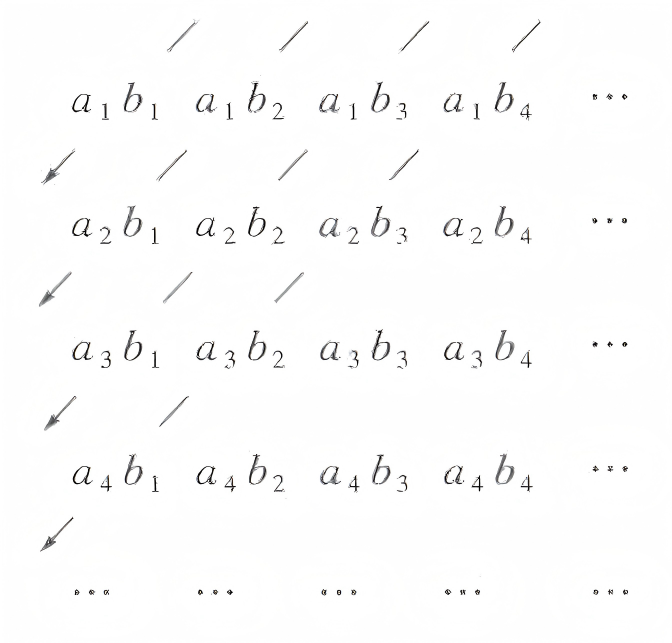
\includegraphics[width=0.4\linewidth]{figure/cauchy(1)}
\end{center}


\[
\begin{aligned}
	c_1 &= a_1 b_1 \\
	c_2 &= a_2 b_1 + a_1 b_2 \\
	&\vdots \\
	c_n &= \sum_{k=1}^n a_k b_{n+1-k}
\end{aligned}
\]
称之为 Cauchy 乘积

2.  正方形排列
\begin{center}
	\centering
	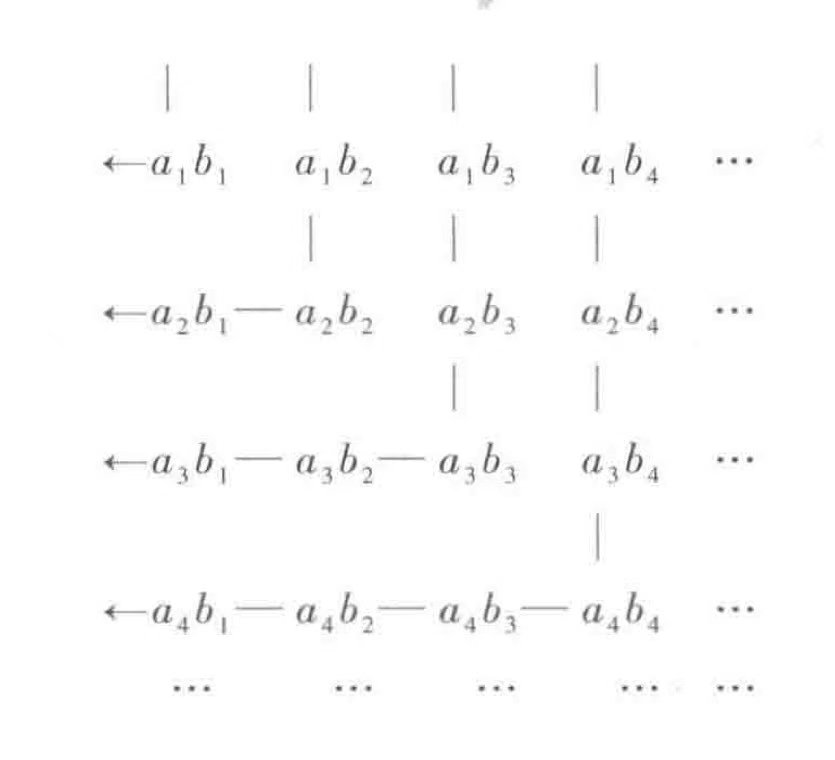
\includegraphics[width=0.4\linewidth]{figure/cubve}
\end{center}


\[
\begin{aligned}
	d_1 &= a_1 b_1 \\
	d_2 &= a_2 b_1 + a_2 b_2 + a_1 b_2 \\
	&\vdots \\
	d_n &= \sum_{k=1}^{n-1} a_n b_k + \sum_{k=1}^{n-1} a_k b_n + a_n b_n
\end{aligned}
\]
其部分和满足：
\[
\sum_{k=1}^n d_k = (a_1 + a_2 + \dots + a_n)(b_1 + b_2 + \dots + b_n)
\]

若级数 $\sum a_n$ 与 $\sum b_n$ 都收敛，则正方形排列的乘积级数 $\sum d_n$ 收敛。设 $\sum a_n = S$，$\sum b_n = T$，则 $\sum d_n = ST$。

但对于 Cauchy 乘积 $\sum c_n$，有可能发散。例如，级数 $\displaystyle \sum_{n=1}^{\infty} \frac{(-1)^{n+1}}{\sqrt{n}}$ 与自身的 Cauchy 乘积发散，而正方形排列的乘积级数收敛。
\begin{proposition}
	（绝对收敛级数的乘积定理）若级数 $\sum a_n$ 与 $\sum b_n$ 都绝对收敛，则将所有乘积项 $a_i b_j$（$i=1,2,\dots; j=1,2,\dots$）按任意方式排列求和而成的级数也绝对收敛，且其和等于
	\[
	\left( \sum_{n=1}^{\infty} a_n \right) \left( \sum_{n=1}^{\infty} b_n \right)
	\]
\end{proposition}
\begin{proof}
	设 $a_{i_k} b_{j_k}$（$k=1,2,\dots$）是所有 $a_i b_j$（$i=1,2,\dots; j=1,2,\dots$）的任意一种排列。对任意正整数 $n$，取
	\[
	N = \max_{1 \le k \le n} \{i_k, j_k\}
	\]
	则
	\[
	\sum_{k=1}^n |a_{i_k} b_{j_k}| \le \sum_{i=1}^N |a_i| \cdot \sum_{i=1}^N |b_i| \le \sum_{n=1}^{\infty} |a_n| \cdot \sum_{n=1}^{\infty} |b_n|
	\]
	因此，级数 $\sum a_{i_k} b_{j_k}$ 绝对收敛。根据绝对收敛级数的重排不变性，其任意更序级数也收敛，且和不变。
	
	设 $\sum d_n$ 是正方形排列下的乘积级数，则 $\sum d_n$ 是 $\sum a_{i_k} b_{j_k}$ 重排后得到的级数。于是
	\[
	\sum_{k=1}^{\infty} a_{i_k} b_{j_k} = \sum_{n=1}^{\infty} d_n = \left( \sum_{n=1}^{\infty} a_n \right) \left( \sum_{n=1}^{\infty} b_n \right)
	\]
\end{proof}
%
% 第5节：无穷乘积
% !TEX root = ../../../main.tex
% 所属：第一部分：单变量分析学 / 第5章：级数理论
% 节：5.5 无穷乘积
% 正文按原文件顺序保存；由 ../chapter5.tex 调用。
\section{无穷乘积}
\begin{definition}
	对数列 $\{p_n\}_{n=1}^{+\infty}$，且对所有 $n \ge 1$，$p_n \neq 0$，称
	\[
	p_1 p_2 \cdots p_n \cdots = \prod_{n=1}^{\infty} p_n
	\]
	为无穷乘积。定义其部分积数列为 $\{P_n\}$：
	\[
	\begin{aligned}
		P_1 &= p_1 \\
		P_2 &= p_1 p_2 \\
		P_3 &= p_1 p_2 p_3 \\
		&\vdots \\
		P_n &= p_1 p_2 \cdots p_n
	\end{aligned}
	\]
	
	若部分积数列 $\{P_n\}$ 收敛于某非零有限数 $P$，则称无穷乘积 $\displaystyle \prod_{n=1}^{\infty} p_n$ 收敛，并称 $P$ 为它的积，记为
	\[
	\prod_{n=1}^{\infty} p_n = P
	\]
	
	若 $\{P_n\}$ 发散，或 $\{P_n\}$ 收敛于 $0$，则称无穷乘积 $\displaystyle \prod_{n=1}^{\infty} p_n$ 发散。
\end{definition}
\begin{proposition}
	若无穷乘积 $\displaystyle \prod_{n=1}^{\infty} p_n$ 收敛，则
	\[
	\lim_{n \to \infty} p_n = 1
	\]
\end{proposition}
\begin{proof}
	设 $\displaystyle \prod_{n=1}^{\infty} p_n = P \neq 0$，那么
	\[
	\lim_{n \to \infty} p_n = \lim_{n \to \infty} \frac{P_n}{P_{n-1}} = \frac{P}{P} = 1
	\]
\end{proof}



从而，我们通常将 $p_n$ 写成 $1 + a_n$ 的形式，即
\[
\prod_{n=1}^{\infty} p_n = \prod_{n=1}^{\infty} (1 + a_n)
\]
由上述命题，若 $\displaystyle \prod_{n=1}^{\infty} p_n$ 收敛，则必有 $a_n \to 0$。

当 $n$ 充分大时，总有 $1 + a_n > 0$，而前有限项不影响无穷乘积的敛散性。因此，下面我们假设：
\begin{itemize}
	\item  对所有 $n$，$1 + a_n > 0$（即 $p_n > 0$）；
	
	\item $a_n \to 0$（即 $p_n \to 1$）。
\end{itemize}
在上述假设下，我们可以建立无穷乘积与无穷级数之间的关系。
\begin{proposition}\label{无穷乘积与无穷级数之间的关系}
	无穷乘积 $\displaystyle \prod_{n=1}^{\infty} p_n = \prod_{n=1}^{\infty} (1 + a_n)$ 收敛，当且仅当级数 $\displaystyle \sum_{n=1}^{\infty} \ln p_n = \sum_{n=1}^{\infty} \ln(1 + a_n)$ 收敛。
	
\end{proposition}
\begin{proof}
	设无穷乘积 $\prod p_n$ 的部分积为 $P_n$，级数 $\sum \ln p_n$ 的部分和为 $S_n$，则有
	\[
	\ln P_n = S_n \quad \Longleftrightarrow \quad P_n = e^{S_n}
	\]
	若 $S_n \to S$ 存在且有限，则 $\lim\limits_{n \to \infty} P_n = e^S$ 存在且有限，故 $\prod p_n$ 收敛。
	反之，若 $P_n \to P$ 存在、有限且大于 $0$，则 $\lim\limits_{n \to \infty} S_n = \ln P$ 存在且有限。
\end{proof}

\begin{corollary}\label{无穷乘积收敛}
	若对所有 $n \ge 1$，$a_n > 0$（或 $a_n < 0$），则无穷乘积 $\displaystyle \prod_{n=1}^{\infty} (1 + a_n)$ 收敛，当且仅当级数 $\displaystyle \sum_{n=1}^{\infty} a_n$ 收敛。
	
\end{corollary}
\begin{proof}
	考虑级数 $\sum \ln(1 + a_n)$ 与 $\sum a_n$。
	若对所有 $n \ge 1$，$a_n > 0$，则 $\ln(1 + a_n) > 0$。
	又因为
	\[
	\lim_{n \to \infty} \frac{\ln(1 + a_n)}{a_n} = 1 \quad (a_n \to 0)
	\]
	由正项级数的比较判别法，$\sum \ln(1 + a_n)$ 与 $\sum a_n$ 有相同的敛散性。
	而由\ref{无穷乘积与无穷级数之间的关系}，$\prod(1 + a_n)$ 与 $\sum \ln(1 + a_n)$ 有相同的敛散性，因此 $\prod(1 + a_n)$ 与 $\sum a_n$ 有相同的敛散性。
	
\end{proof}
\begin{corollary}
	对任意项级数 $\sum a_n$，若 $\sum a_n$ 收敛，则无穷乘积 $\displaystyle \prod_{n=1}^{\infty} (1 + a_n)$ 收敛，当且仅当 $\displaystyle \sum_{n=1}^{\infty} a_n^2$ 收敛。
	
\end{corollary}
\begin{proof}
	由不等式 $\ln(1 + a_n) \le a_n$，可得 $a_n - \ln(1 + a_n) \ge 0$。
	计算极限：
	\[
	\lim_{n \to \infty} \frac{a_n - \ln(1 + a_n)}{a_n^2} = \lim_{x \to 0} \frac{x - \ln(1 + x)}{x^2} = \frac{1}{2}
	\]
	故正项级数 $\sum (a_n - \ln(1 + a_n))$ 与 $\sum a_n^2$ 有相同的敛散性。
	
	若 $\prod(1 + a_n)$ 收敛，则由\ref{无穷乘积与无穷级数之间的关系}，$\sum \ln(1 + a_n)$ 收敛。又已知 $\sum a_n$ 收敛，故 $\sum (a_n - \ln(1 + a_n))$ 收敛，从而 $\sum a_n^2$ 收敛。反之同理可证。
\end{proof}
\begin{definition}
	若级数 $\sum \ln p_n = \sum \ln(1 + a_n)$ 绝对收敛，就称无穷乘积 $\displaystyle \prod_{n=1}^{\infty} p_n = \prod_{n=1}^{\infty} (1 + a_n)$ 绝对收敛。
\end{definition}
\begin{proposition}
	下面三个说法等价：
	\begin{enumerate}
		\item 无穷乘积 $\displaystyle \prod_{n=1}^{\infty} (1 + a_n)$ 绝对收敛；
		\item 无穷乘积 $\displaystyle \prod_{n=1}^{\infty} (1 + |a_n|)$ 收敛；
		\item 级数 $\displaystyle \sum_{n=1}^{\infty} |a_n|$ 收敛。
	\end{enumerate}
\end{proposition}
\begin{proof}
	由\ref{无穷乘积与无穷级数之间的关系}，$\prod(1 + |a_n|)$ 收敛当且仅当 $\sum \ln(1 + |a_n|)$ 收敛。又因为 $|a_n| \ge 0$，由推论 \ref{无穷乘积收敛}，$\sum \ln(1 + |a_n|)$ 收敛当且仅当 $\sum |a_n|$ 收敛，故 2 $\iff$ 3。
	
	下证 1 $\iff$ 3：
	根据定义，$\prod(1 + a_n)$ 绝对收敛 $\iff$ $\sum |\ln(1 + a_n)|$ 收敛。
	考虑极限：
	\[
	\lim_{n \to \infty} \frac{|\ln(1 + a_n)|}{|a_n|} = 1
	\]
	由正项级数的比较判别法，$\sum |\ln(1 + a_n)|$ 与 $\sum |a_n|$ 有相同的敛散性。因此 1 $\iff$ 3。
	
	综上，1、2、3 三个命题等价。
\end{proof}

下面介绍著名的 Wallis 公式与 Stirling 公式，涉及了一定的定积分，读者可以在读完定积分后再读，现在只需记下公式就足够了。
\begin{proposition}（Wallis 公式）
	设 \( p_n = 1 - \dfrac{1}{(2n)^2} \)，则
	\[
	\prod_{n=1}^{\infty} p_n = \frac{2}{\pi}
	\]
\end{proposition}
\begin{proof}
	\[
	\begin{aligned}
		P_n &= \prod_{k=1}^{n} \left(1 - \frac{1}{(2k)^2}\right)
		= \prod_{k=1}^{n} \frac{(2k-1)(2k+1)}{(2k)(2k)} \\
		&= \frac{1 \cdot 3 \cdot 3 \cdot \cdots \cdot (2n-1)(2n+1)}{2 \cdot 2 \cdot 4 \cdot 4 \cdot \cdots \cdot (2n)(2n)}
		= \frac{[(2n-1)!!]^2}{[(2n)!!]^2} \cdot (2n+1)
	\end{aligned}
	\]
	
	考虑定积分 \( I_n = \displaystyle\int_{0}^{\pi/2} \sin^n x \dd x \)。
	后面我们将知道：
	\[
	I_{2n} = \frac{(2n-1)!!}{(2n)!!} \cdot \frac{\pi}{2}, \quad I_{2n+1} = \frac{(2n)!!}{(2n+1)!!}
	\]
	因此
	\[
	\frac{\pi}{2} P_n = \frac{I_{2n}}{I_{2n+1}}
	\]
	
	由不等式 \( I_{2n+1} < I_{2n} < I_{2n-1} \)，得
	\[
	1 < \frac{I_{2n}}{I_{2n+1}} < \frac{I_{2n-1}}{I_{2n+1}}
	\]
	因为
	\[
	\lim_{n \to \infty} \frac{I_{2n-1}}{I_{2n+1}} = \lim_{n \to \infty} \frac{2n+1}{2n} = 1
	\]
	由夹逼性，
	\[
	\lim_{n \to \infty} P_n = \lim_{n \to \infty} \left( \frac{2}{\pi} \cdot \frac{I_{2n}}{I_{2n+1}} \right) = \frac{2}{\pi}
	\]
	故
	\[
	\prod_{n=1}^{\infty} \left(1 - \frac{1}{(2n)^2}\right) = \frac{2}{\pi}
	\]
\end{proof}


换一个形式，就是 Wallis 公式：
\[
\frac{\pi}{2} = \frac{2}{1} \cdot \frac{2}{3} \cdot \frac{4}{3} \cdot \frac{4}{5} \cdot \cdots \cdot \frac{2n}{2n-1} \cdot \frac{2n}{2n+1} \cdot \cdots
\]
\begin{proposition}
	（Stirling 公式）
	\[
	n! \sim \sqrt{2\pi n} \left( \frac{n}{e} \right)^n \quad (n \to +\infty)
	\]
	
\end{proposition}
\begin{proof}
	设 \( b_n = \dfrac{n! e^n}{n^{n+1/2}}, \ n=1,2,\dots \)，则
	\[
	\begin{aligned}
		\frac{b_n}{b_{n-1}} &= e\left(1 - \frac{1}{n}\right)^{n - \frac{1}{2}}
		= \exp\left[1 + \left(n - \frac{1}{2}\right)\ln\left(1 - \frac{1}{n}\right)\right] \\
		&= \exp\left( -\frac{1}{12n^2} + o\left(\frac{1}{n^2}\right) \right)
		= 1 - \frac{1}{12n^2} + o\left(\frac{1}{n^2}\right)
	\end{aligned}
	\]
	
	令 \( 1 + a_n = \dfrac{b_n}{b_{n-1}} \)，于是 \( \sum a_n \) 收敛。那么
	\[
	\prod_{n=2}^{\infty} (1 + a_n) = \prod_{n=2}^{\infty} \frac{b_n}{b_{n-1}}
	\]
	收敛，因此 \( \lim\limits_{n \to \infty} b_n = b_1 \displaystyle\prod_{n=2}^{\infty} \dfrac{b_n}{b_{n-1}} = A \neq 0 \)。
	
	利用 Wallis 公式：
	\[
	A = \lim_{n \to \infty} b_n = \lim_{n \to \infty} \frac{b_n^2}{b_{2n}}
	= \lim_{n \to \infty} \frac{(2n)!!}{(2n-1)!!} \cdot \sqrt{\frac{2}{n}} = \sqrt{2\pi}
	\]
	因此得到 Stirling 公式：
	\[
	n! \sim \sqrt{2\pi n} \left( \frac{n}{e} \right)^n
	\]
\end{proof}
\begin{example}
	证明
	\[
	\sin x=x\prod_{n=1}^{\infty}\left(1-\frac{x^2}{n^2\pi^2}\right).
	\]
\end{example}

\begin{proof}
	由三角函数的知识,我们知道
	\[
	\sin 3\varphi=\sin\varphi\left(3-4\sin^2\varphi\right),
	\]
	\[
	\sin 5\varphi=\sin\varphi\left(5-20\sin^2\varphi+16\sin^4\varphi\right).
	\]
	利用三角恒等式
	\[
	\sin(2k+1)\varphi
	=2(1-2\sin^2\varphi)\sin(2k-1)\varphi-\sin(2k-3)\varphi,
	\]
	以及应用数学归纳法,可以得到
	\[
	\sin(2n+1)\varphi=\sin\varphi\,P(\sin^2\varphi),
	\tag{*}
	\]
	其中 $P(u)$ 是 $n$ 次多项式,它的常数项为
	\[
	P(0)=\lim_{\varphi\to0}\frac{\sin(2n+1)\varphi}{\sin\varphi}=2n+1.
	\]
	由于
	\[
	\varphi=\frac{k\pi}{2n+1}\quad(k=1,2,\cdots,n)
	\]
	使 $(*)$ 式的左端成为 $0$,且
	\[
	\sin^2\frac{k\pi}{2n+1}\quad(k=1,2,\cdots,n)
	\]
	给出 $P(u)$ 的 $n$ 个不同的根,于是
	\[
	P(u)=(2n+1)\prod_{k=1}^{n}
	\left(1-\frac{u}{\sin^2\dfrac{k\pi}{2n+1}}\right).
	\]
	从而得到
	\[
	\sin(2n+1)\varphi
	=(2n+1)\sin\varphi\prod_{k=1}^{n}
	\left(1-\frac{\sin^2\varphi}{\sin^2\dfrac{k\pi}{2n+1}}\right).
	\]
	令 $x=(2n+1)\varphi$,代入后得到
	\[
	\sin x
	=(2n+1)\sin\frac{x}{2n+1}\prod_{k=1}^{n}
	\left(1-\frac{\sin^2\dfrac{x}{2n+1}}{\sin^2\dfrac{k\pi}{2n+1}}\right).
	\]
	因此,当 $m<n$ 时,成立
	\[
	\frac{\sin x}
	{(2n+1)\sin\dfrac{x}{2n+1}
		\displaystyle\prod_{k=1}^{m}
		\left(1-\frac{\sin^2\dfrac{x}{2n+1}}{\sin^2\dfrac{k\pi}{2n+1}}\right)}
	=
	\prod_{k=m+1}^{n}
	\left(1-\frac{\sin^2\dfrac{x}{2n+1}}{\sin^2\dfrac{k\pi}{2n+1}}\right).
	\tag{**}
	\]
	当 $n\to\infty$ 时,$(**)$ 式左端的极限为
	\[
	\frac{\sin x}{x\displaystyle\prod_{k=1}^{m}
		\left(1-\frac{x^2}{k^2\pi^2}\right)}.
	\]
	另一方面,取 $m$ 充分大,使得 $m>|x|/2$.由于
	\[
	\sin^2\frac{x}{2n+1}<\frac{x^2}{(2n+1)^2},
	\]
	并且当 $1\leq k\leq n$ 时,
	\[
	\sin^2\frac{k\pi}{2n+1}
	\geq \frac{4}{\pi^2}\frac{k^2\pi^2}{(2n+1)^2}
	=\frac{4k^2}{(2n+1)^2},
	\]
	故关于 $(**)$ 式的右端,有估计式
	\[
	\begin{aligned}
		1
		&>\prod_{k=m+1}^{n}
		\left(1-\frac{\sin^2\dfrac{x}{2n+1}}{\sin^2\dfrac{k\pi}{2n+1}}\right) \\
		&\geq \prod_{k=m+1}^{n}\left(1-\frac{x^2}{4k^2}\right)
		\geq \prod_{k=m+1}^{\infty}\left(1-\frac{x^2}{4k^2}\right).
	\end{aligned}
	\]
	令 $n\to\infty$,就得到
	\[
	1\geq
	\frac{\sin x}{x\displaystyle\prod_{k=1}^{m}
		\left(1-\frac{x^2}{k^2\pi^2}\right)}
	\geq
	\prod_{k=m+1}^{\infty}\left(1-\frac{x^2}{4k^2}\right).
	\]
	由级数 $\displaystyle\sum_{k=m+1}^{\infty}\frac{x^2}{4k^2}$ 的收敛性,可知无穷乘积
	\[
	\prod_{k=m+1}^{\infty}\left(1-\frac{x^2}{4k^2}\right)
	\]
	收敛,并且当 $m\to\infty$ 时,上述尾乘积趋于 $1$.根据夹逼性,得到
	\[
	\lim_{m\to\infty}
	\frac{\sin x}{x\displaystyle\prod_{k=1}^{m}
		\left(1-\frac{x^2}{k^2\pi^2}\right)}=1.
	\]
	于是
	\[
	\sin x=x\prod_{k=1}^{\infty}\left(1-\frac{x^2}{k^2\pi^2}\right).
	\]
	当 $x=0$ 或 $x=\pm n\pi$ 时,两端显然同为 $0$,故结论对所有 $x$ 成立.
\end{proof}






%
